\chapter{Qué es una imagen para una computadora}
\label{cap:imagen}

\begin{enpocas}
Píxeles y canales de color, cómo forma una imagen una cámara (modelo estenopeico), qué es el campo de
visión, qué ve la cámara del dron y cómo se pasa de un píxel a un punto del mundo.
\end{enpocas}

\section{Una imagen es una tabla de números}

Para nosotros una foto es una escena; para la computadora es una \textbf{tabla de números}. La cámara
del dron entrega imágenes de 640 columnas por 480 filas: 307\,200 \textbf{píxeles} (de \emph{picture
element}). Cada píxel tiene tres números entre 0 y 255: cuánto rojo, cuánto verde y cuánto azul (RGB).
$(0,0,0)$ es negro, $(255,255,255)$ blanco y $(230,140,55)$ un naranja de fuego.

\begin{figure}[H]
\centering
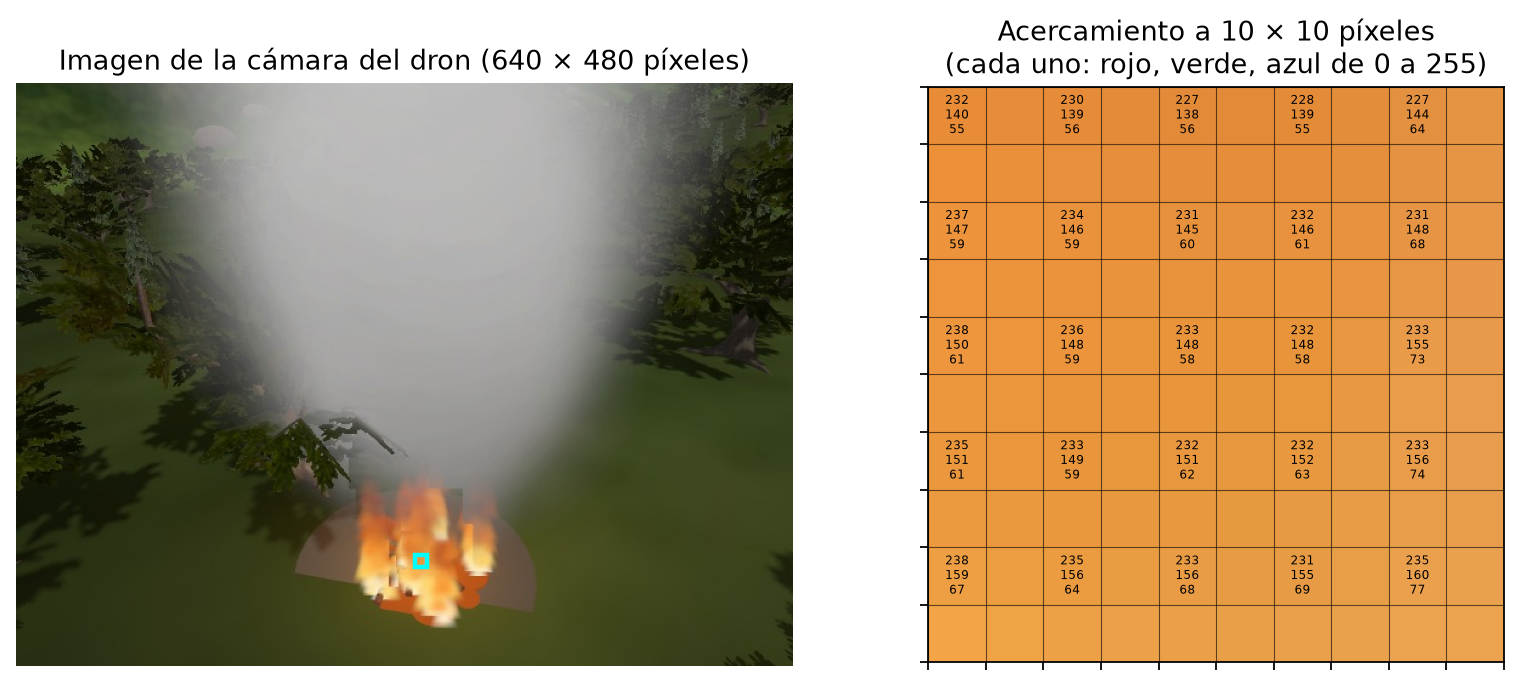
\includegraphics[width=\textwidth]{c_pixeles.png}
\caption{Una imagen de la cámara del dron y un acercamiento a 10$\times$10 píxeles de las llamas:
mucho rojo (230), algo de verde (145) y poco azul (60).}
\label{fig:pixeles}
\end{figure}

Las tres tablas (rojo, verde, azul) se llaman \textbf{canales}. Verlas por separado ayuda a entender
por qué el fuego es fácil de distinguir: brilla mucho en el canal rojo y poco en el azul, mientras que
el humo es claro en los tres.

\begin{figure}[H]
\centering
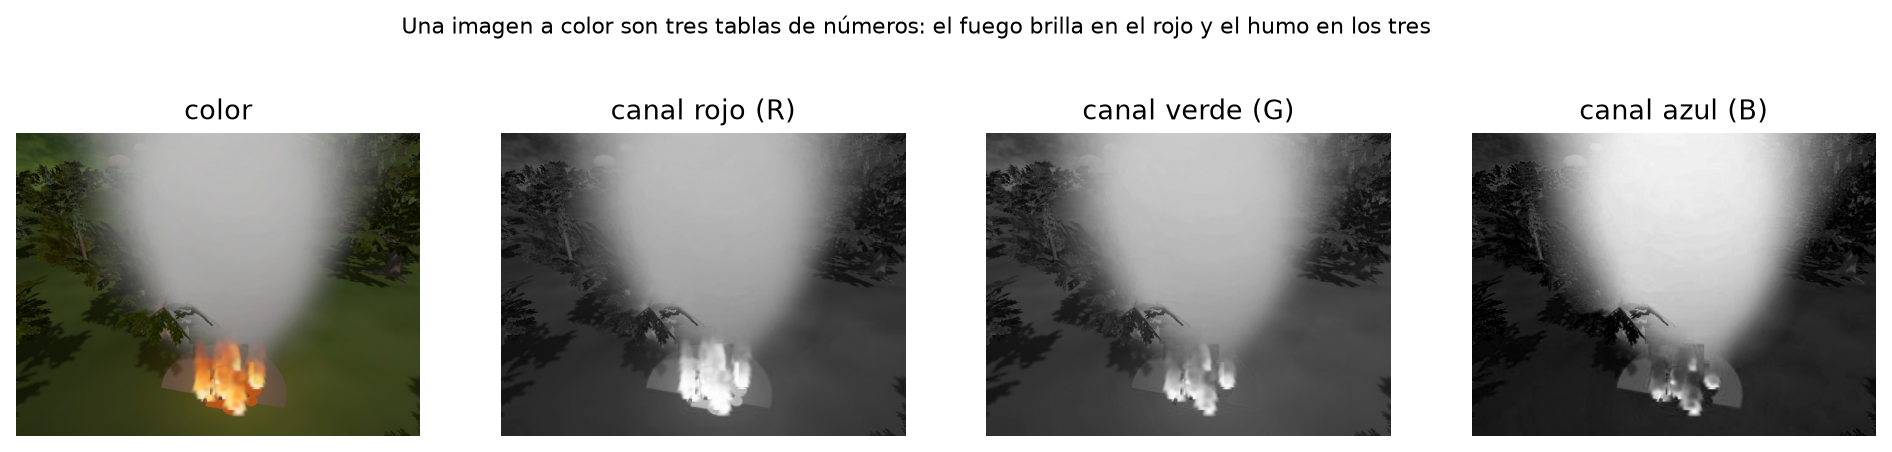
\includegraphics[width=\textwidth]{c_rgb.png}
\caption{La misma imagen separada en sus tres canales (más claro = valor más alto).}
\end{figure}

\begin{ejemplo}
Una imagen es como una hoja de cálculo gigante donde cada celda está pintada de un color. Un programa
de visión ``lee'' esa hoja buscando patrones de números, igual que tú buscarías un patrón de colores.
\end{ejemplo}

Un video son imágenes una tras otra: la cámara simulada entrega 15 por segundo en el tópico
\cod{/cuadrirotor/camara}.

\section{Cómo forma una imagen una cámara}

El modelo más útil es el de la \textbf{cámara estenopeica} (\emph{pinhole}): una caja oscura con un
agujerito. La luz de cada punto del mundo entra en línea recta por el agujero y llega a un punto del
sensor. Por semejanza de triángulos, un punto a distancia $Z$ y desplazado $X$ del eje aparece en la
imagen a
\begin{equation}
u = f\,\frac{X}{Z},
\end{equation}
donde $f$ es la \textbf{distancia focal} (en píxeles). Los objetos lejanos se ven más pequeños:
dividir entre $Z$ es la \emph{perspectiva}.

\begin{figure}[H]
\centering
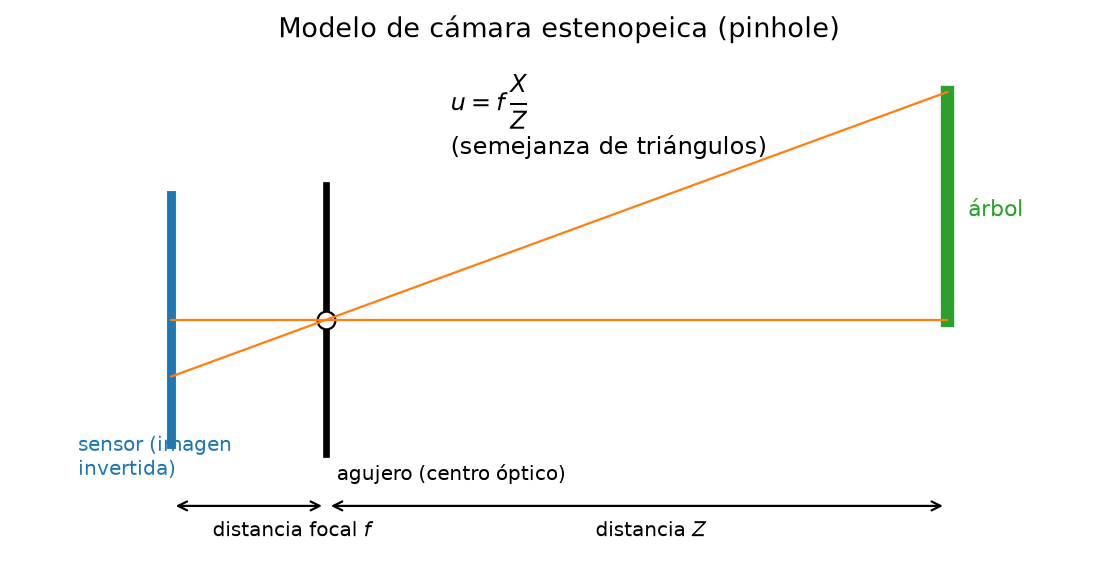
\includegraphics[width=0.85\textwidth]{c_estenopeica.png}
\caption{El modelo estenopeico: la imagen se forma por rayos rectos que pasan por el centro óptico.}
\end{figure}

\section{Campo de visión}

El \textbf{campo de visión} (FOV) es qué tan ancho ve la cámara. La del dron tiene un campo horizontal
de 1.3~rad (74°); con una imagen de 640 píxeles de ancho eso da
\begin{equation}
f = \frac{640/2}{\tan(1.3/2)} \approx 418\ \text{píxeles}.
\end{equation}
Va inclinada 30° hacia abajo: así ve el horizonte (para descubrir humo lejos) y también el suelo
delante del dron.

\begin{figure}[H]
\centering
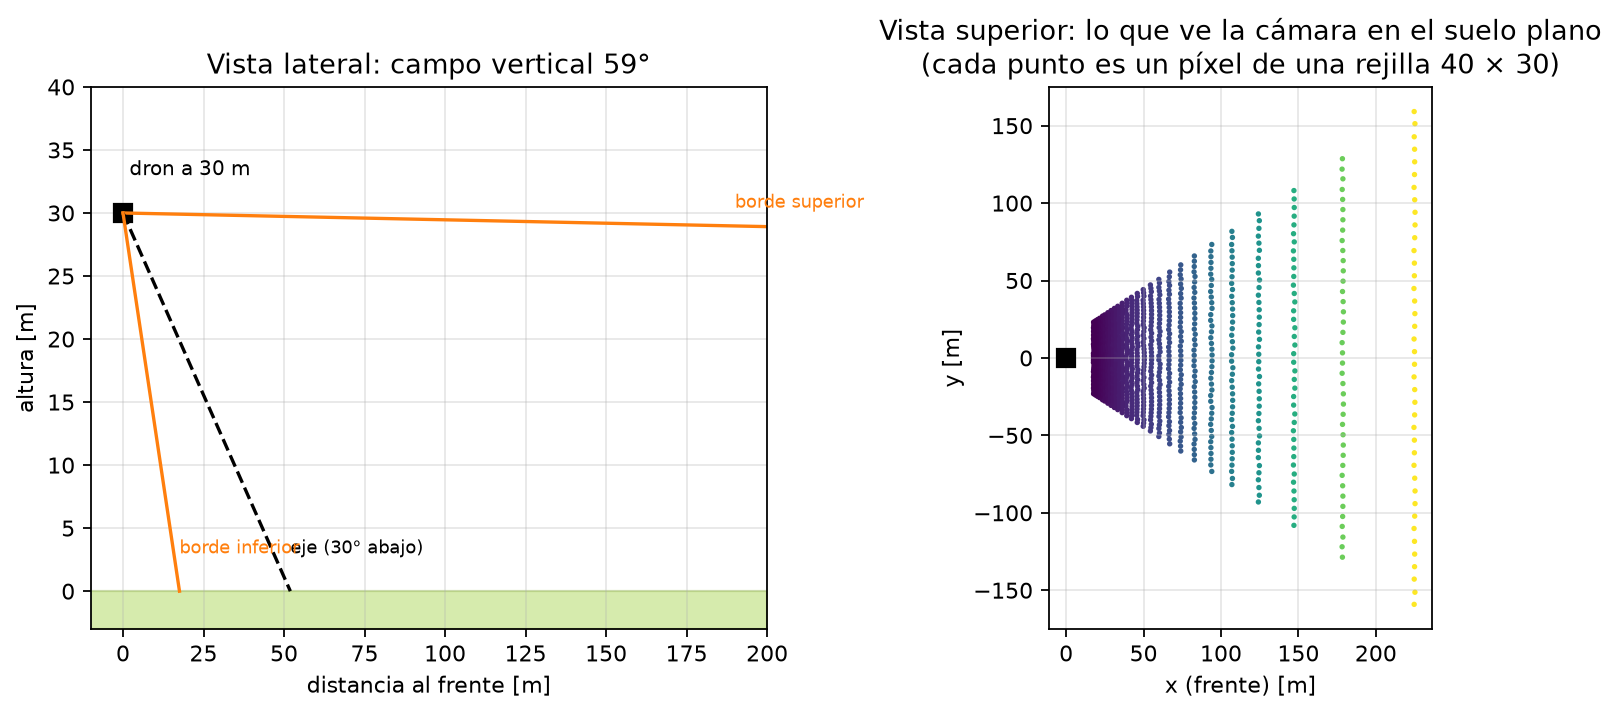
\includegraphics[width=\textwidth]{c_fov.png}
\caption{Qué ve la cámara desde 30~m de altura. Izquierda: el borde superior de la imagen casi toca
el horizonte y el inferior cae a 18~m del dron. Derecha: la ``huella'' de la imagen en el suelo; los
píxeles de arriba cubren mucho más terreno que los de abajo.}
\label{fig:fov}
\end{figure}

\begin{figure}[H]
\centering
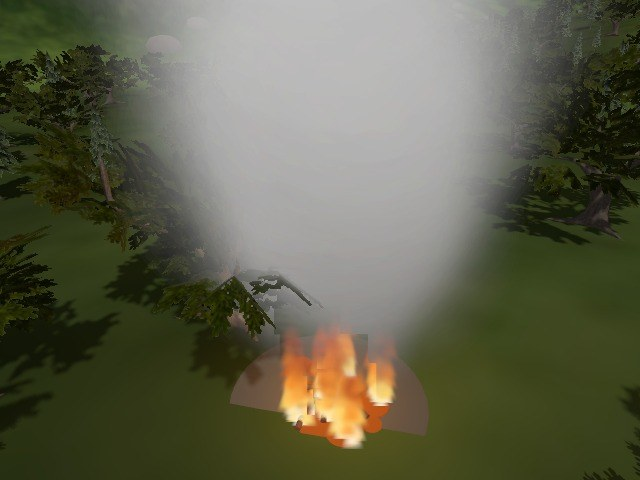
\includegraphics[width=0.32\textwidth]{ds_fuego_humo.jpg}\hfill
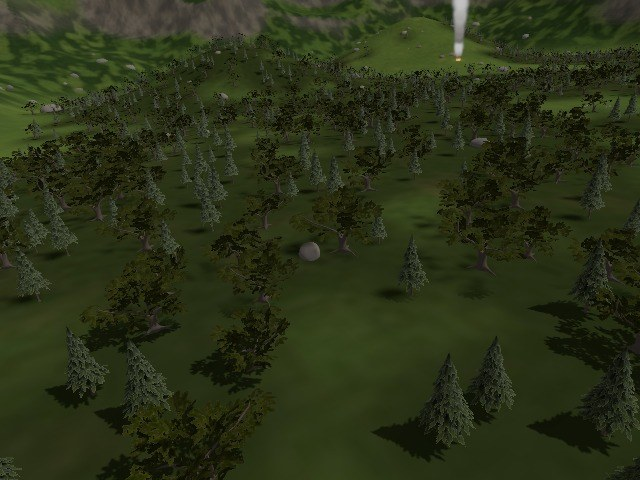
\includegraphics[width=0.32\textwidth]{ds_humo_lejano.jpg}\hfill
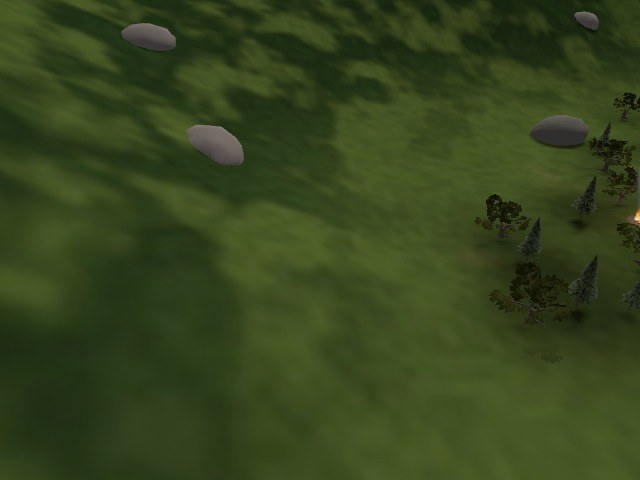
\includegraphics[width=0.32\textwidth]{ds_sin_fuego.jpg}
\caption{Imágenes de la cámara del dron simulado: fuego y humo de cerca, humo a lo lejos (la columna
blanca arriba a la derecha) y una escena sin fuego con rocas.}
\end{figure}

\section{Del píxel al mundo: rayos}

La cámara pierde una dimensión: un píxel no dice a qué distancia está lo que muestra, solo en qué
\emph{dirección}. Cada píxel corresponde a un \textbf{rayo} que sale de la cámara. Invirtiendo el
modelo estenopeico, el rayo del píxel $(u,v)$ en el marco de la cámara es
\begin{equation}
d_{cam} = \Big(1,\ -\frac{u - W/2}{f},\ -\frac{v - H/2}{f}\Big),
\end{equation}
y se pasa al mundo con la orientación del dron y de la cámara. Para saber \emph{dónde} está lo que se
ve, hace falta otra información:
\begin{itemize}
  \item un modelo del terreno: el punto está donde el rayo toca el suelo (así se estima el fuego,
        capítulo~\ref{cap:conceptos-autonomia});
  \item o varias vistas desde lugares distintos: donde se cruzan los rayos (triangulación, como se
        hace con el humo).
\end{itemize}

\begin{recuerda}
Una cámara da direcciones, no distancias. Para ubicar algo en el mapa hay que cruzar su rayo con el
terreno o con otros rayos.
\end{recuerda}
